\part{Supplemental Advanced Topics}

\chapter{Subpixel Rendering Algorithms}

\section{ClearType Technology}

\begin{definitionbox}{ClearType Overview}
ClearType (Microsoft) leverages RGB subpixel geometry to achieve 3× horizontal resolution for grayscale content, particularly text rendering.
\end{definitionbox}

\begin{figure}[H]
\centering
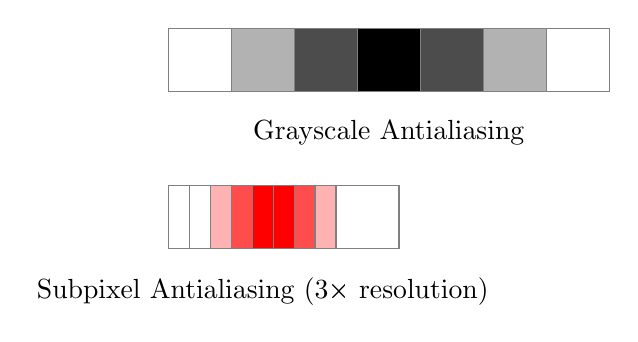
\begin{tikzpicture}[scale=0.8]
  % Traditional grayscale antialiasing
  \begin{scope}
    \foreach \x/\col in {0/0, 1/30, 2/70, 3/100, 4/70, 5/30, 6/0} {
      \fill[black!\col] (\x,0) rectangle +(1,1);
      \draw[gray] (\x,0) rectangle +(1,1);
    }
    \node[below] at (3.5,-0.3) {Grayscale Antialiasing};
  \end{scope}
  
  % Subpixel rendering
  \begin{scope}[yshift=-2.5cm]
    \foreach \x/\r/\g/\b in {
      0/0/0/0,
      1/0/10/30,
      2/30/50/70,
      3/70/90/100,
      4/100/100/100,
      5/100/90/70,
      6/70/50/30,
      7/30/10/0,
      8/0/0/0
    } {
      \fill[red!\r] (\x*0.333,0) rectangle +(0.333,1);
      \fill[green!\g] (\x*0.333+0.333,0) rectangle +(0.333,1);
      \fill[blue!\b] (\x*0.333+0.666,0) rectangle +(0.333,1);
      \draw[gray,thin] (\x*0.333,0) rectangle +(0.999,1);
    }
    \node[below] at (1.5,-0.3) {Subpixel Antialiasing (3× resolution)};
  \end{scope}
\end{tikzpicture}
\caption{Comparison of grayscale vs subpixel antialiasing. Subpixel rendering achieves 3× horizontal resolution.}
\end{figure}

\subsection{Mathematical Model}

\begin{formulabox}{ClearType Algorithm}
\textbf{Step 1:} Generate oversampled grayscale image at 3× horizontal resolution

\textbf{Step 2:} Apply asymmetric filter $F$ accounting for subpixel order:
\begin{equation}
  F = [0.06, 0.24, 0.40, 0.24, 0.06] \quad \text{(normalized Gaussian)}
\end{equation}

\textbf{Step 3:} Distribute filtered values to RGB subpixels:
\begin{align}
  R(x,y) &= F_R(G_{\text{oversample}}) \\
  G(x,y) &= F_G(G_{\text{oversample}}) \\
  B(x,y) &= F_B(G_{\text{oversample}})
\end{align}
\end{formulabox}

\section{Implementation Considerations}

\begin{itemize}
  \item Requires knowledge of subpixel order (RGB vs BGR)
  \item Rotation-dependent (only works for horizontal text)
  \item Can introduce color fringes on high-contrast edges
  \item Ineffective on PenTile due to shared subpixels
\end{itemize}

